\begin{figure}[H]
\centering
\includegraphics[page=8,width=0.44\textwidth]{\FCNCFigures/tthML/showFake/faketau/prefit/NOMINAL/reg1l1tau1b1j_ss_vetobtagwp70_highmet/tau_pt_0.pdf}
%\put(-100, 140){\textbf{(a)}}
%\put(-120, 130){\footnotesize{$l\thad 1j$}}
\includegraphics[page=8,width=0.44\textwidth]{\FCNCFigures/tthML/showFake/faketau/prefit/NOMINAL/reg1l1tau1b2j_ss_vetobtagwp70_highmet/tau_pt_0.pdf}
%\put(-100, 140){\textbf{(b)}}
%\put(-120, 130){\footnotesize{$l\thad 2j$}}

\includegraphics[page=8,width=0.44\textwidth]{\FCNCFigures/tthML/showFake/faketau/prefit/NOMINAL/reg1l1tau1b2j_os_vetobtagwp70_highmet/tau_pt_0.pdf}
%\put(-100, 140){\textbf{(c)}}
%\put(-120, 130){\footnotesize{$t_h	lhad$-2j}}
\includegraphics[page=8,width=0.44\textwidth]{\FCNCFigures/tthML/showFake/faketau/prefit/NOMINAL/reg1l1tau1b3j_os_vetobtagwp70_highmet/tau_pt_0.pdf}
%\put(-100, 140){\textbf{(d)}}
%\put(-120, 130){\footnotesize{$t_h	lhad$-3j}}

\includegraphics[page=8,width=0.44\textwidth]{\FCNCFigures/tthML/showFake/faketau/prefit/NOMINAL/reg1l2tau1bnj_os/tau_pt_0.pdf}
%\put(-100, 140){\textbf{(e)}}
%\put(-120, 130){\footnotesize{$l\thadhad$}}
\caption{ The distributions of $\tau$ $\pt$ in the signal regions of leptonic channel with fake tau origin shown. Only statistical uncertainties are being shown. Underflow and overflow bins are included respectively in the first and last bins. The real tau contributions shown from ttbar and other MC including diboson, single top, and V+jets.}
\label{fig:wjet_pt}
\end{figure}
